\section*{Generating multinormal and multi-student r.v.'s}

\subsection*{Q1}

First we run the following script:

\begin{verbatim}
> set.seed(1)
> sum(duplicated(runif(1e6))) ## = 120
[1] 120
> sum(duplicated(rnorm(1e8))) ## = 0
[1] 0
\end{verbatim}

The function \verb|duplicated| returns a logical array where unique numbers are marked with 0 and duplicates are marked with 1 (the first occurence of the number is marked with a 0). Summming this array thus gives the total number of duplicates. The uniform distribution gives 120 duplicates in a much smaller sample size than the normal distribution, which gives 0 duplicates.

In the assignment, the expected number of different numbers is derived to be 
\begin{displaymath}
  \E[N_n] = \frac{1 - f^n}{1-f}
\end{displaymath}

The number of duplicates is then given by 
$n - \E[N_n]$
We run the following script:

\begin{verbatim}
> m <- 2^32;n <- 1e6
> f <- 1 - 1/m
> num_dup_unif <- n - (1-f^n)/(1-f)
> num_dup_unif
[1] 116.3988
\end{verbatim}

The expected result of 116.4 is quite close to the generated result. The outcome of 120 is therefore consistent with the assumption that \verb|runif| produces different values uniformly.

The resolution of \verb|rnorm| is somewhere in the $2^{50}$'s. Directly calculating $1 - f^n$ will give $1$, because f is so close to $1$.
First, we use to approximation given in the assignment.
\begin{displaymath}
f^n = \left( 1 - \frac{1}{m}\right)^n \approx 1 - \frac{n}{m} + \frac{n^2}{2m^2}
\end{displaymath}

Inserting this into our equation for the number of different numbers gives
\begin{displaymath}
\frac{1 - f^n}{1-f} \approx \frac{1 - 1 + \frac{n}{m} - \frac{n^2}{2m^2}}{1- \left(1 - \frac{1}{m}\right)}  = \frac{\frac{n}{m} - \frac{n^2}{2m^2}}{\frac{1}{m}} = n - \frac{n^2}{2m}
\end{displaymath}

This results in the following equation for the expected number of duplicates.
\begin{displaymath}
n - \left(n - \frac{n^2}{2m}\right) = \frac{n^2}{2m}
\end{displaymath}

Next we check in \verb|R| if the number of duplicates is consistent with values for $m$ of $10^{15}$, $10^{16}$, $10^{17}$ or $10^{18}$, when $n$ is $10^8$
\begin{verbatim}
> n_norm <- 1e8
> m_norm <- c(1e15,1e16,1e17,1e18)
> num_dup_norm <- n_norm^2/(2*m_norm)
> num_dup_norm
[1] 5.000 0.500 0.050 0.005
\end{verbatim}

The obtained result seems to be consistent with a resolution of $10^{16}$ or higher.
 
\subsection*{Q2}
The following code is executed in \verb|R|.
\begin{verbatim}
> n <- 200; p <- 0.52
> x <- c(0,cumsum(2*rbinom(n,1,p)-1))
> plot(x, type="l", lwd=1, ylab="state", xlab="step", main="1-dimensional random walk")
\end{verbatim}
This gives the following biased random walk:

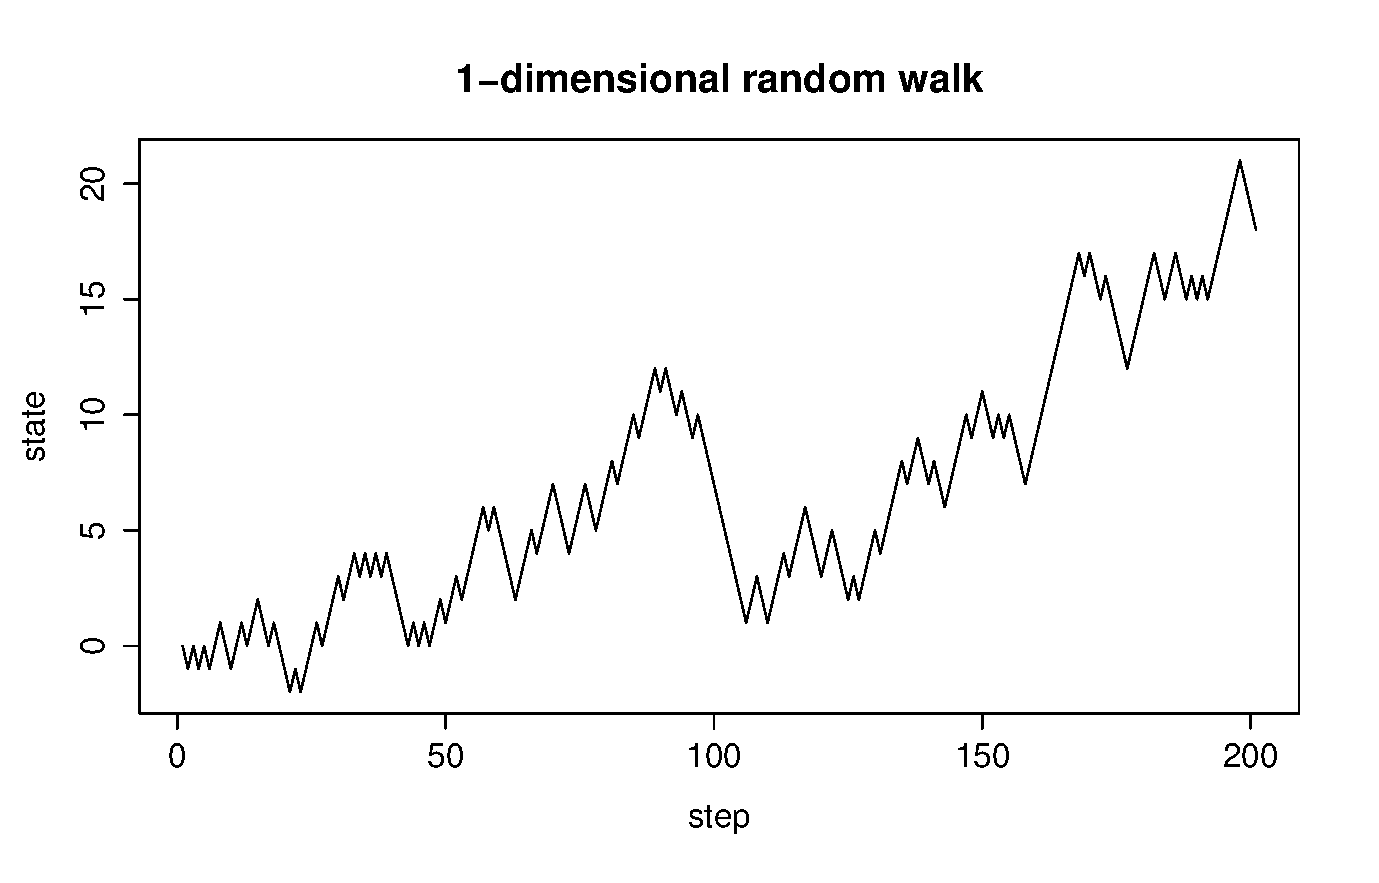
\includegraphics[scale=.6]{NL1_Q2_1D-randomwalk.eps} 

\subsection*{Q3}

Given that $X$, $Y \sim N(0,1)$, we want to transform $(X, Y)$ into $(X, Y^*)$, with $Y^* = aX + bY$, with $a, b$ chosen in such a way that $\Var[Y^*] = 1$ and $r(X, Y^*) = 0.8$.

\begin{align*}
r(X, Y^*) & = \frac{\E[X Y^*] - \E[X] \E[Y*]}{\sqrt{\Var[X] \Var[Y^*]}} = \frac{\E[a X^2 + b X Y] - 0 \cdot \E[Y^*]}{\sqrt{1 * 1}} \\
          & = a * \E[X^2] + b * \E[X Y] = a (\Var[X] - \E[X]^2) = a
\end{align*}

Here we use that $\E[X] = 0$, $\Var[X] = \Var[Y] = \Var[Y^*] = 1$. Also $\E[X Y] = \E[X] \E[]Y] = 0$, because $X$ and $Y$ are independent.
Next we use the condition that the variance of $Y^*$ must also be 1.

\begin{displaymath}
\Var[Y^*] = \Var[aX + bY] = a^2 \Var[X] + b^2 \Var[Y] + 2ab \Cov[X,Y] = a^2 + b^2 = 1
\end{displaymath}

We can conclude from this that $a = 0.8$ and $b = \sqrt{1 - a^2} = 0.6$.

In \verb|R| code:

\begin{verbatim}
set.seed(2004); options(digits=2)
X <- rnorm(1000); Y <- rnorm(1000)
a <- .8; b <- sqrt(1 - a^2); Y <- a*X + b*Y
\end{verbatim}

\subsection*{Q4}

The variance-covariance matrix $\Sigma$ of the random vector $(X, Y^*)$ is equal to the correlation matrix because $\Var[X] = \Var[Y^*] = 1$. It is given by the following expression.

\begin{displaymath}
\Sigma = 
\begin{pmatrix}
\Cov[X,X] & \Cov[X, Y^*] \\
\Cov[Y^*,X] & \Cov[Y^*, Y^*]
\end{pmatrix}
=
\begin{pmatrix}
\Var[X] & r(X,Y^*) \\
r(X, Y^*) & \Var[Y^*]
\end{pmatrix}
=
\begin{pmatrix}
1 & 0.8 \\
0.8 & 1
\end{pmatrix}
\end{displaymath}

\subsection*{Q5}
If $A$ is to be the Cholesky decomposition of $\Sigma$, it should be a lower triangular matrix with real and positive entries and $A A^* = \Sigma$, where $A^*$ is the conjugate transpose of $A$. Checking this gives

\begin{displaymath}
\begin{pmatrix}
1 & 0 \\
a & b
\end{pmatrix}
\begin{pmatrix}
1 & a \\
0 & b
\end{pmatrix}
=
\begin{pmatrix}
1 & a \\
a & a^2 + b^2
\end{pmatrix}
=
\begin{pmatrix}
1 & a \\
a & 1
\end{pmatrix}
=
\begin{pmatrix}
1 & 0.8 \\
0.8 & 1
\end{pmatrix}
= \Sigma
\end{displaymath}

\subsection*{Q6}
We execute the following \verb|R| code.
\begin{verbatim}
> c(mean(X), var(X), mean(Y), var(Y), cor(X,Y))
[1] 0.051 0.983 0.070 0.994 0.796
\end{verbatim}

The means of $X$ and $Y^*$ are close to $0$. The variances close to $1$ and the correlation is close to $0.8$. This resembles the theoretical values quite close.

\subsection*{Q7}
Let $(X, Y)$ be bivariate Normal with $\E[X] = \E[Y] = 0$, $\Var[X] = \Var[Y] = 1$ and $r(X,Y) = r$. $W$ is independent of $(X, Y)$. Then

\begin{align*}
r(XW, YW) & = \frac{\E[XWYW] - \E[XW]\E[YW]}{\sqrt{\Var[XW] \Var[YW]}} \\
	      & = \frac{\E[W^2]\E[XY] - \E[W]^2\E[X]\E[Y]}{\sqrt{\left(\E[W^2]\E[X^2] - \E[W]^2\E[X]^2\right)\left(\E[W^2]\E[Y^2] - \E[W]^2\E[Y]^2\right)}} \\
	      & = \frac{\E[W]^2\E[XY] - 0}{\sqrt{\left(\E[W^2]\E[X^2] - 0\right)\left(\E[W^2]\E[Y^2] - 0\right)}} \\ 
	      & = \frac{\E[W^2]}{\sqrt{\E[W^2]^2}} \frac{\E[XY]}{\Var[X]\Var[Y]} = r \cdot \frac{\E[W^2]}{\sqrt{\E[W^2]^2}} = r
\end{align*}

When $\E[W^2]$ is finite, the final step in the derivation is allowed. This is equivalent with demanding $\Var[W]$ to be finite.

\subsection*{Q8}

Next, we execute the following \verb|R| code.

\begin{verbatim}
> chi5 <- sqrt(rchisq(1000, df=5)/5)
> X <- X/chi5; Y <- Y/chi5 
> c(mean(X), var(X), mean(Y), var(Y), cor(X,Y))
[1] 0.038 1.525 0.068 1.528 0.786
\end{verbatim}

We take $X$ and $Y*$ as defined earlier. $V \sim \chi^2_k$ and $W = \sqrt{k/V}$ with $k=5$.  The population mean of $XW$ is $0$ because $\E[XW] = \E[X]\E[W] = 0$. The same holds for $Y^{*}W$. $r(XW,Y^{*}W) = 0.8$ has been proven in question $7$.
Next we determine the variance of $XW$.
\begin{align*}
\Var[XW] & = \E[X]^2 \Var[W] + \Var[X] \E[W]^2 + \Var[X]\Var[W] \\
         & =  0 + \Var[X](\E[W]^2 + \Var[W]) = \Var[X]\E[W^2] \\
         & = 1 \cdot \E[k/V] = k \E[1/V]
\end{align*}